\PassOptionsToPackage{unicode=true}{hyperref} % options for packages loaded elsewhere
\PassOptionsToPackage{hyphens}{url}
%
\documentclass[
]{book}
\usepackage{lmodern}
\usepackage{amssymb,amsmath}
\usepackage{ifxetex,ifluatex}
\ifnum 0\ifxetex 1\fi\ifluatex 1\fi=0 % if pdftex
  \usepackage[T1]{fontenc}
  \usepackage[utf8]{inputenc}
  \usepackage{textcomp} % provides euro and other symbols
\else % if luatex or xelatex
  \usepackage{unicode-math}
  \defaultfontfeatures{Scale=MatchLowercase}
  \defaultfontfeatures[\rmfamily]{Ligatures=TeX,Scale=1}
\fi
% use upquote if available, for straight quotes in verbatim environments
\IfFileExists{upquote.sty}{\usepackage{upquote}}{}
\IfFileExists{microtype.sty}{% use microtype if available
  \usepackage[]{microtype}
  \UseMicrotypeSet[protrusion]{basicmath} % disable protrusion for tt fonts
}{}
\makeatletter
\@ifundefined{KOMAClassName}{% if non-KOMA class
  \IfFileExists{parskip.sty}{%
    \usepackage{parskip}
  }{% else
    \setlength{\parindent}{0pt}
    \setlength{\parskip}{6pt plus 2pt minus 1pt}}
}{% if KOMA class
  \KOMAoptions{parskip=half}}
\makeatother
\usepackage{xcolor}
\IfFileExists{xurl.sty}{\usepackage{xurl}}{} % add URL line breaks if available
\IfFileExists{bookmark.sty}{\usepackage{bookmark}}{\usepackage{hyperref}}
\hypersetup{
  pdftitle={Postgraduate Research Methods and Analysis},
  pdfauthor={Christopher J. Wilson},
  pdfborder={0 0 0},
  breaklinks=true}
\urlstyle{same}  % don't use monospace font for urls
\usepackage{color}
\usepackage{fancyvrb}
\newcommand{\VerbBar}{|}
\newcommand{\VERB}{\Verb[commandchars=\\\{\}]}
\DefineVerbatimEnvironment{Highlighting}{Verbatim}{commandchars=\\\{\}}
% Add ',fontsize=\small' for more characters per line
\usepackage{framed}
\definecolor{shadecolor}{RGB}{248,248,248}
\newenvironment{Shaded}{\begin{snugshade}}{\end{snugshade}}
\newcommand{\AlertTok}[1]{\textcolor[rgb]{0.94,0.16,0.16}{#1}}
\newcommand{\AnnotationTok}[1]{\textcolor[rgb]{0.56,0.35,0.01}{\textbf{\textit{#1}}}}
\newcommand{\AttributeTok}[1]{\textcolor[rgb]{0.77,0.63,0.00}{#1}}
\newcommand{\BaseNTok}[1]{\textcolor[rgb]{0.00,0.00,0.81}{#1}}
\newcommand{\BuiltInTok}[1]{#1}
\newcommand{\CharTok}[1]{\textcolor[rgb]{0.31,0.60,0.02}{#1}}
\newcommand{\CommentTok}[1]{\textcolor[rgb]{0.56,0.35,0.01}{\textit{#1}}}
\newcommand{\CommentVarTok}[1]{\textcolor[rgb]{0.56,0.35,0.01}{\textbf{\textit{#1}}}}
\newcommand{\ConstantTok}[1]{\textcolor[rgb]{0.00,0.00,0.00}{#1}}
\newcommand{\ControlFlowTok}[1]{\textcolor[rgb]{0.13,0.29,0.53}{\textbf{#1}}}
\newcommand{\DataTypeTok}[1]{\textcolor[rgb]{0.13,0.29,0.53}{#1}}
\newcommand{\DecValTok}[1]{\textcolor[rgb]{0.00,0.00,0.81}{#1}}
\newcommand{\DocumentationTok}[1]{\textcolor[rgb]{0.56,0.35,0.01}{\textbf{\textit{#1}}}}
\newcommand{\ErrorTok}[1]{\textcolor[rgb]{0.64,0.00,0.00}{\textbf{#1}}}
\newcommand{\ExtensionTok}[1]{#1}
\newcommand{\FloatTok}[1]{\textcolor[rgb]{0.00,0.00,0.81}{#1}}
\newcommand{\FunctionTok}[1]{\textcolor[rgb]{0.00,0.00,0.00}{#1}}
\newcommand{\ImportTok}[1]{#1}
\newcommand{\InformationTok}[1]{\textcolor[rgb]{0.56,0.35,0.01}{\textbf{\textit{#1}}}}
\newcommand{\KeywordTok}[1]{\textcolor[rgb]{0.13,0.29,0.53}{\textbf{#1}}}
\newcommand{\NormalTok}[1]{#1}
\newcommand{\OperatorTok}[1]{\textcolor[rgb]{0.81,0.36,0.00}{\textbf{#1}}}
\newcommand{\OtherTok}[1]{\textcolor[rgb]{0.56,0.35,0.01}{#1}}
\newcommand{\PreprocessorTok}[1]{\textcolor[rgb]{0.56,0.35,0.01}{\textit{#1}}}
\newcommand{\RegionMarkerTok}[1]{#1}
\newcommand{\SpecialCharTok}[1]{\textcolor[rgb]{0.00,0.00,0.00}{#1}}
\newcommand{\SpecialStringTok}[1]{\textcolor[rgb]{0.31,0.60,0.02}{#1}}
\newcommand{\StringTok}[1]{\textcolor[rgb]{0.31,0.60,0.02}{#1}}
\newcommand{\VariableTok}[1]{\textcolor[rgb]{0.00,0.00,0.00}{#1}}
\newcommand{\VerbatimStringTok}[1]{\textcolor[rgb]{0.31,0.60,0.02}{#1}}
\newcommand{\WarningTok}[1]{\textcolor[rgb]{0.56,0.35,0.01}{\textbf{\textit{#1}}}}
\usepackage{longtable,booktabs}
% Allow footnotes in longtable head/foot
\IfFileExists{footnotehyper.sty}{\usepackage{footnotehyper}}{\usepackage{footnote}}
\makesavenoteenv{longtable}
\usepackage{graphicx,grffile}
\makeatletter
\def\maxwidth{\ifdim\Gin@nat@width>\linewidth\linewidth\else\Gin@nat@width\fi}
\def\maxheight{\ifdim\Gin@nat@height>\textheight\textheight\else\Gin@nat@height\fi}
\makeatother
% Scale images if necessary, so that they will not overflow the page
% margins by default, and it is still possible to overwrite the defaults
% using explicit options in \includegraphics[width, height, ...]{}
\setkeys{Gin}{width=\maxwidth,height=\maxheight,keepaspectratio}
\setlength{\emergencystretch}{3em}  % prevent overfull lines
\providecommand{\tightlist}{%
  \setlength{\itemsep}{0pt}\setlength{\parskip}{0pt}}
\setcounter{secnumdepth}{5}
% Redefines (sub)paragraphs to behave more like sections
\ifx\paragraph\undefined\else
  \let\oldparagraph\paragraph
  \renewcommand{\paragraph}[1]{\oldparagraph{#1}\mbox{}}
\fi
\ifx\subparagraph\undefined\else
  \let\oldsubparagraph\subparagraph
  \renewcommand{\subparagraph}[1]{\oldsubparagraph{#1}\mbox{}}
\fi

% set default figure placement to htbp
\makeatletter
\def\fps@figure{htbp}
\makeatother

\usepackage{booktabs}
\usepackage[]{natbib}
\bibliographystyle{apalike}

\title{Postgraduate Research Methods and Analysis}
\author{Christopher J. Wilson}
\date{2020-09-03}

\begin{document}
\maketitle

{
\setcounter{tocdepth}{1}
\tableofcontents
}
\hypertarget{welcome-to-the-module}{%
\chapter{Welcome to the module}\label{welcome-to-the-module}}

\hypertarget{module-overview}{%
\chapter{Module Overview}\label{module-overview}}

This Level 7 module for first year Doctorate in Clinical Psychology trainees aims to enable you to:

\begin{itemize}
\tightlist
\item
  Refresh and extend your knowledge, skills and critical understanding of advanced research methods using both qualitative and quantitative approaches;
\item
  Creatively apply the principles of quantitative and qualitative research methods to clinical psychology research and practice;
\item
  Refresh and extend your skills in project design, management, analysis and presentation.
\end{itemize}

The module is also designed to explicitly prepare you for the two Doctorate level research modules which occur in Years Two and Three of the programme, ensuring that you have the requisite knowledge and skills to successfully engage with those modules.

The key foci for this module include:

\begin{itemize}
\tightlist
\item
  critical review of established literature
\item
  project design
\item
  project management
\item
  data analysis
\item
  dissemination of research findings
\end{itemize}

The module is taught using a variety of techniques to best enhance your knowledge and understanding of the application of research theory and methods in the context of clinical psychology. These include lectures, seminars, guided statistical analysis and tutorials with the latter being used to provide individual guidance and formative feedback. The module has its own site on the University's Virtual Learning Environment \url{http://eat.tees.ac.uk} - known as Blackboard), with resources and literature designed to support learning.

\hypertarget{module-timetable-and-delivery-for-20202021}{%
\section{Module timetable and delivery for 2020/2021}\label{module-timetable-and-delivery-for-20202021}}

The timetable for this module appears on the Clinical Psychology Programme Site/Timetables.
The majority of the sessions will take place on Monday mornings. Please note that the timetable should be checked on a regular basis.

\textbf{Due to COVID19 pandemic, the sessions for this module will be delivered online in 2020/21}

\hypertarget{learning-and-teaching-strategies}{%
\section{Learning and Teaching Strategies}\label{learning-and-teaching-strategies}}

The module is taught using a variety of techniques to best enhance your knowledge and understanding of the application of research theory and methods in the context of clinical psychology. This includes activities designed to encourage independent learning, a key skill for successful performance in research modules in Years Two and Three of the programme. Evidence of independent learning is expected in the assignments for this module. Specific links are made with research informed activity in practice.

You will be provided with two papers for critical review at the start of the module and asked to decide which one you will use for your summative critical review assignment; one of these papers is from a quantitative research tradition and the other is from a qualitative research tradition.

All presentations (with added annotations) are available, along with additional support materials, via an \href{mailto:e-learning@tees}{\nolinkurl{e-learning@tees}} on the VLE. E-learning is enabled through group activities on the VLE or Microsoft Teams where discussion and problem solving is undertaken in relation to tasks set during teaching sessions. The discussion boards or Microsoft Teams site will be used to ask and answer questions that arise from the taught material and also your independent work.

\hypertarget{how-will-the-online-sessions-work}{%
\section{How will the online sessions work?}\label{how-will-the-online-sessions-work}}

The video below explains how online sessions will work:

\hypertarget{assessment}{%
\chapter{Assessment}\label{assessment}}

\hypertarget{formative-assessment}{%
\section{Formative assessment}\label{formative-assessment}}

Formative feedback is provided throughout the module through practical exercises and in seminars on trainee presentations.

By the end of year one, trainees are expected to have identified a thesis topic and have a completed research proposal. As such, there are a number of formative milestones across the year that will be monitored by the module team. Please see Appendix 1 of this guide for details.

The required format for thesis research proposals can be found in Appendix 2 of the DClinPsy
Programme Research Handbook.

\textbf{The formal formative assessment is of a presentation of the thesis research proposal to be presented during the research panels, which take place on 20, 21 and 22 July 2020.} The presentation will be 20 minutes' long and will outline the thesis project that the trainee will develop in Years 2 and 3. There will also be 10 minutes allotted for questions from the panel which will have two academic members and one clinical member. This formative assessment is intended as a starting point for the Year 2 and 3 research methods modules. The timing is important as it should enable trainees to start the process of ethics approval for their dissertation. earlier. The trainees will hand in a printed copy of their slides with explanatory notes and references.

\textbf{Formative Assessment Criteria}

The following criteria will be used to assess the assignment:

\begin{itemize}
\tightlist
\item
  Effective justification for the study.
\item
  Clearly defined research question.
\item
  Comprehensive and critical review of the literature (within time constraints).
\item
  Realistic research design.
\item
  Effective consideration of ethical issues.
\item
  Clear plan for writing up and dissemination.
\item
  Fulfilment of professional research ethics requirements.
\item
  Adherence to the relevant guidance for presentation as advised by the Module Tutor.
\end{itemize}

\hypertarget{summative-assessments}{%
\section{Summative Assessments}\label{summative-assessments}}

Assessment consists of an ICA and an ECA, each worth 50\% of the overall module mark. The deadlines for these assessments can be found in the assessments section on Blackboard or in the programme assessment timetable.

\textbf{ICA (50\%)} - A critical review of a published primary research paper (choice to be made by a trainee from three papers with different methodologies provided by the tutor). One of these papers is from a quantitative research approach, one from a qualitative research approach and the third will use mixed methods (2,000 words).
\emph{Learning outcomes: (KU 1-4, CIS 1-3, KTS 1-3)}

\textbf{ICA Assessment Criteria (Critical Appraisal of Published Primary Research Paper )}

The following criteria will be used to assess the assignment:

\begin{itemize}
\tightlist
\item
  Demonstrate a critical understanding of the role of the reviewed paper for clinical psychologists in service delivery and/or practice.
\item
  Demonstrate a critical and comprehensive understanding of the relevant methodological issues.
\item
  Systematically and critically evaluate stages of the research process.
\item
  Demonstrate a comprehensive and critical understanding of the ethical issues involved in the research.
\item
  Reach effectively argued conclusions.
\item
  Demonstrate independent learning ability through reflection on the critical review process.
\item
  Adhere to the American Psychological Association (APA) guidelines for presentation and referencing.
\end{itemize}

\textbf{ECA (50\%)} - A research project proposal which both addresses limitations identified in the ICA critical review (1) and develops the research further with the use of an alternative methodology (2,000 words).\\
\emph{Learning outcomes: (KU 1-4, CIS 1-3, PPS 1-2, KTS 1-5)}

\textbf{ECA Assessment Criteria (Research Project Proposal)}

The following criteria will be used to assess the assignment:

\begin{itemize}
\tightlist
\item
  Identify a project that demonstrates a detailed and critical understanding of the research evidence reviewed and wider methodological issues, including the role of the project for informing service delivery and/or practice.
\item
  Provide detailed and appropriately justified solutions to the design of the research project.
\item
  Consider both methodological and ethical issues in the design of the research project.
\item
  Demonstrate a detailed and critical understanding of the data analysis required for the proposed study.
\item
  Adhere to the American Psychological Association (APA) guidelines for presentation and referencing.
\end{itemize}

\hypertarget{word-limits-for-assessment}{%
\subsection{Word limits for assessment}\label{word-limits-for-assessment}}

Word limits are as stated above (note that there is no allowance of +10\%). The word count refers to the assignment itself and does not include the reference list or tables/graphs. The references cited in the main body of text are included in the word count.

\hypertarget{submitting-work}{%
\section{Submitting work}\label{submitting-work}}

All work should be submitted electronically, using the apporpriate links on the module Blackboard site. A printed hard copy of the assignment is \textbf{not} required and should not be submitted. \textbf{The university's policy is that all assessments must be submitted by 4 p.m. on the day of the deadline.}

\hypertarget{a-note-about-referencing}{%
\section{A note about referencing}\label{a-note-about-referencing}}

There is an expectation that all academic assignments conform to current American Psychological Association referencing and citation conventions. Poor referencing will be taken into consideration when marking. It is recommended that you use a digital reference management system (e.g., Refworks, Mendley), which are freely available (and will save you time). The following online resources are also useful:

\url{http://reciteworks.com/} - good for checking fine details (e.g., missing references)

\url{http://www.apastyle.org} - detailed guidance for APA style

\url{https://owl.english.purdue.edu/owl/resource/560/01/}- additional advice for APA style

\hypertarget{statistical-analysis-software}{%
\chapter{Statistical analysis software}\label{statistical-analysis-software}}

You may be familiar with SPSS from your undergraduate statistics teaching. Please note that we do not use SPSS for teaching and instead use R Statistics. The reason for this is that R is a free statistical package, meaning that it can be accessed in NHS settings that do not have funding for SPSS. This will enable you to run statistical analyses whilst on placement where required, and also enables you to conduct statistical analyses as a qualified Psychologist without incurring any software costs. R is also more flexible than SPSS and has greater functionality. During the teaching you will be shown how to set up and install R, and how to run statistical analyses in this software.

You can obtain R and R Studio from the following links:

\url{https://cran.r-project.org/}

\url{https://rstudio.com/}

\hypertarget{academic-support-and-guidance}{%
\chapter{Academic Support and Guidance}\label{academic-support-and-guidance}}

Please contact the module team if you have any questions, concerns or any other areas you wish to discuss.

\hypertarget{module-team-contact-details}{%
\section{Module Team Contact Details}\label{module-team-contact-details}}

Module Leader: Dr Christopher Wilson: \href{mailto:christopher.wilson@tees.ac.uk}{\nolinkurl{christopher.wilson@tees.ac.uk}}

Module Team: Dr Alan Bowman: \href{mailto:A.Bowman@tees.ac.uk}{\nolinkurl{A.Bowman@tees.ac.uk}}

Guest lecturers from Schools within the University and Local NHS clinicians also contribute to some teaching

\hypertarget{appendix-1-considering-your-thesis}{%
\chapter{Appendix 1: Considering your thesis}\label{appendix-1-considering-your-thesis}}

Your doctoral thesis is one of the largest pieces of work you will undertake during your training and it is important to start thinking about it early on.

You are advised to read around the area of your thesis topic on a continuing basis, and make use of tutorials with your supervision team when needed.

It is also advised that you consider research governance and ethics as you develop your project. Please speak to your academic supervisor about this as they will be able to advise or direct you to someone with appropriate expertise to address queries.

As specified in the Research Handbook, \textbf{please note that a revised version of your research proposal forms one of your year two summative assignments}. The deadline for this assignment is \textbf{early on in the start of second year} and it is therefore advised that you work on your revised proposal as soon as you receive feedback from the panels and have discussed this with your academic supervisor.

\hypertarget{introduction-to-r-and-r-studio}{%
\chapter{Introduction to R and R Studio}\label{introduction-to-r-and-r-studio}}

\hypertarget{by-the-end-of-this-section-you-should-be-able-to}{%
\section{By the end of this section, you should be able to:}\label{by-the-end-of-this-section-you-should-be-able-to}}

\begin{itemize}
\tightlist
\item
  Download R and R studio
\item
  Identify the R script, R console, Data environment and file browser in R studio
\item
  Write and run R code from a script
\item
  Install and load R packages
\end{itemize}

\hypertarget{why-learn-use-r}{%
\section{Why learn / use R?}\label{why-learn-use-r}}

\hypertarget{some-information-about-r}{%
\subsection{Some information about R}\label{some-information-about-r}}

\begin{itemize}
\tightlist
\item
  R is developed and used by scientists and researchers around the world
\item
  Open source = no cost
\item
  Constant development
\item
  Connects to other data science/research tools
\item
  Worldwide community: training widely available
\item
  Encourages transparency and reproducibility
\item
  Publication-ready outputs
\end{itemize}

\hypertarget{moving-from-other-software-to-r}{%
\subsection{Moving from other software to R}\label{moving-from-other-software-to-r}}

\begin{itemize}
\tightlist
\item
  Workflow is different

  \begin{itemize}
  \tightlist
  \item
    Organise files and data differently
  \item
    Workspace can contain data and outputs
  \item
    Can manage multiple datasets within a workspace
  \end{itemize}
\item
  Learning curve can be steep initially

  \begin{itemize}
  \tightlist
  \item
    e.g.~Variables and coding, scripts
  \end{itemize}
\item
  Need to know what you want

  \begin{itemize}
  \tightlist
  \item
    e.g.~building your regression model / ANOVA error terms
  \end{itemize}
\end{itemize}

\hypertarget{r-has-many-advantages}{%
\section{R has many advantages}\label{r-has-many-advantages}}

\begin{itemize}
\tightlist
\item
  Using scripts means analysis is easy to follow and reproduce
\item
  R scripts are small, online collaboration, no SPSS ``older version'' problems
\item
  Data can be organised and reorganised however you need it (tidyr)
\item
  Packages are available for ``cutting edge'' analysis: e.g.~Big Data \& Machine Learning
\item
  A robust language for precise plots and graphics (ggplot)
\item
  R analysis code can be embdeded into documents and presentations (R Markdown)
\end{itemize}

\hypertarget{download-r-and-r-studio}{%
\section{Download R and R Studio}\label{download-r-and-r-studio}}

Click on these links to download:

\begin{itemize}
\tightlist
\item
  \href{https://cran.r-project.org/}{R project}
\item
  \href{https://rstudio.com/}{RStudio}
\end{itemize}

\hypertarget{the-r-studio-environment}{%
\section{The R Studio environment}\label{the-r-studio-environment}}

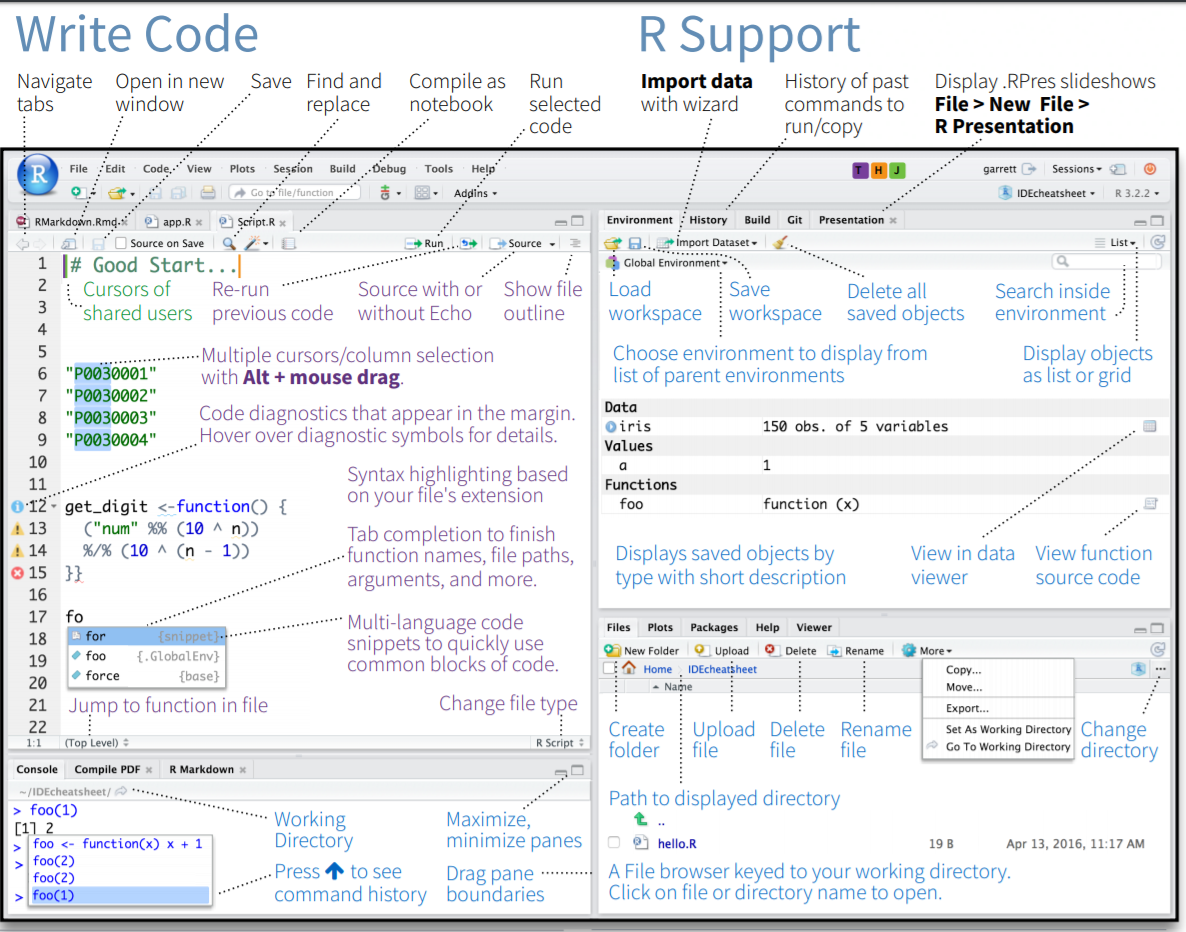
\includegraphics{images/rstudio_ide.png}
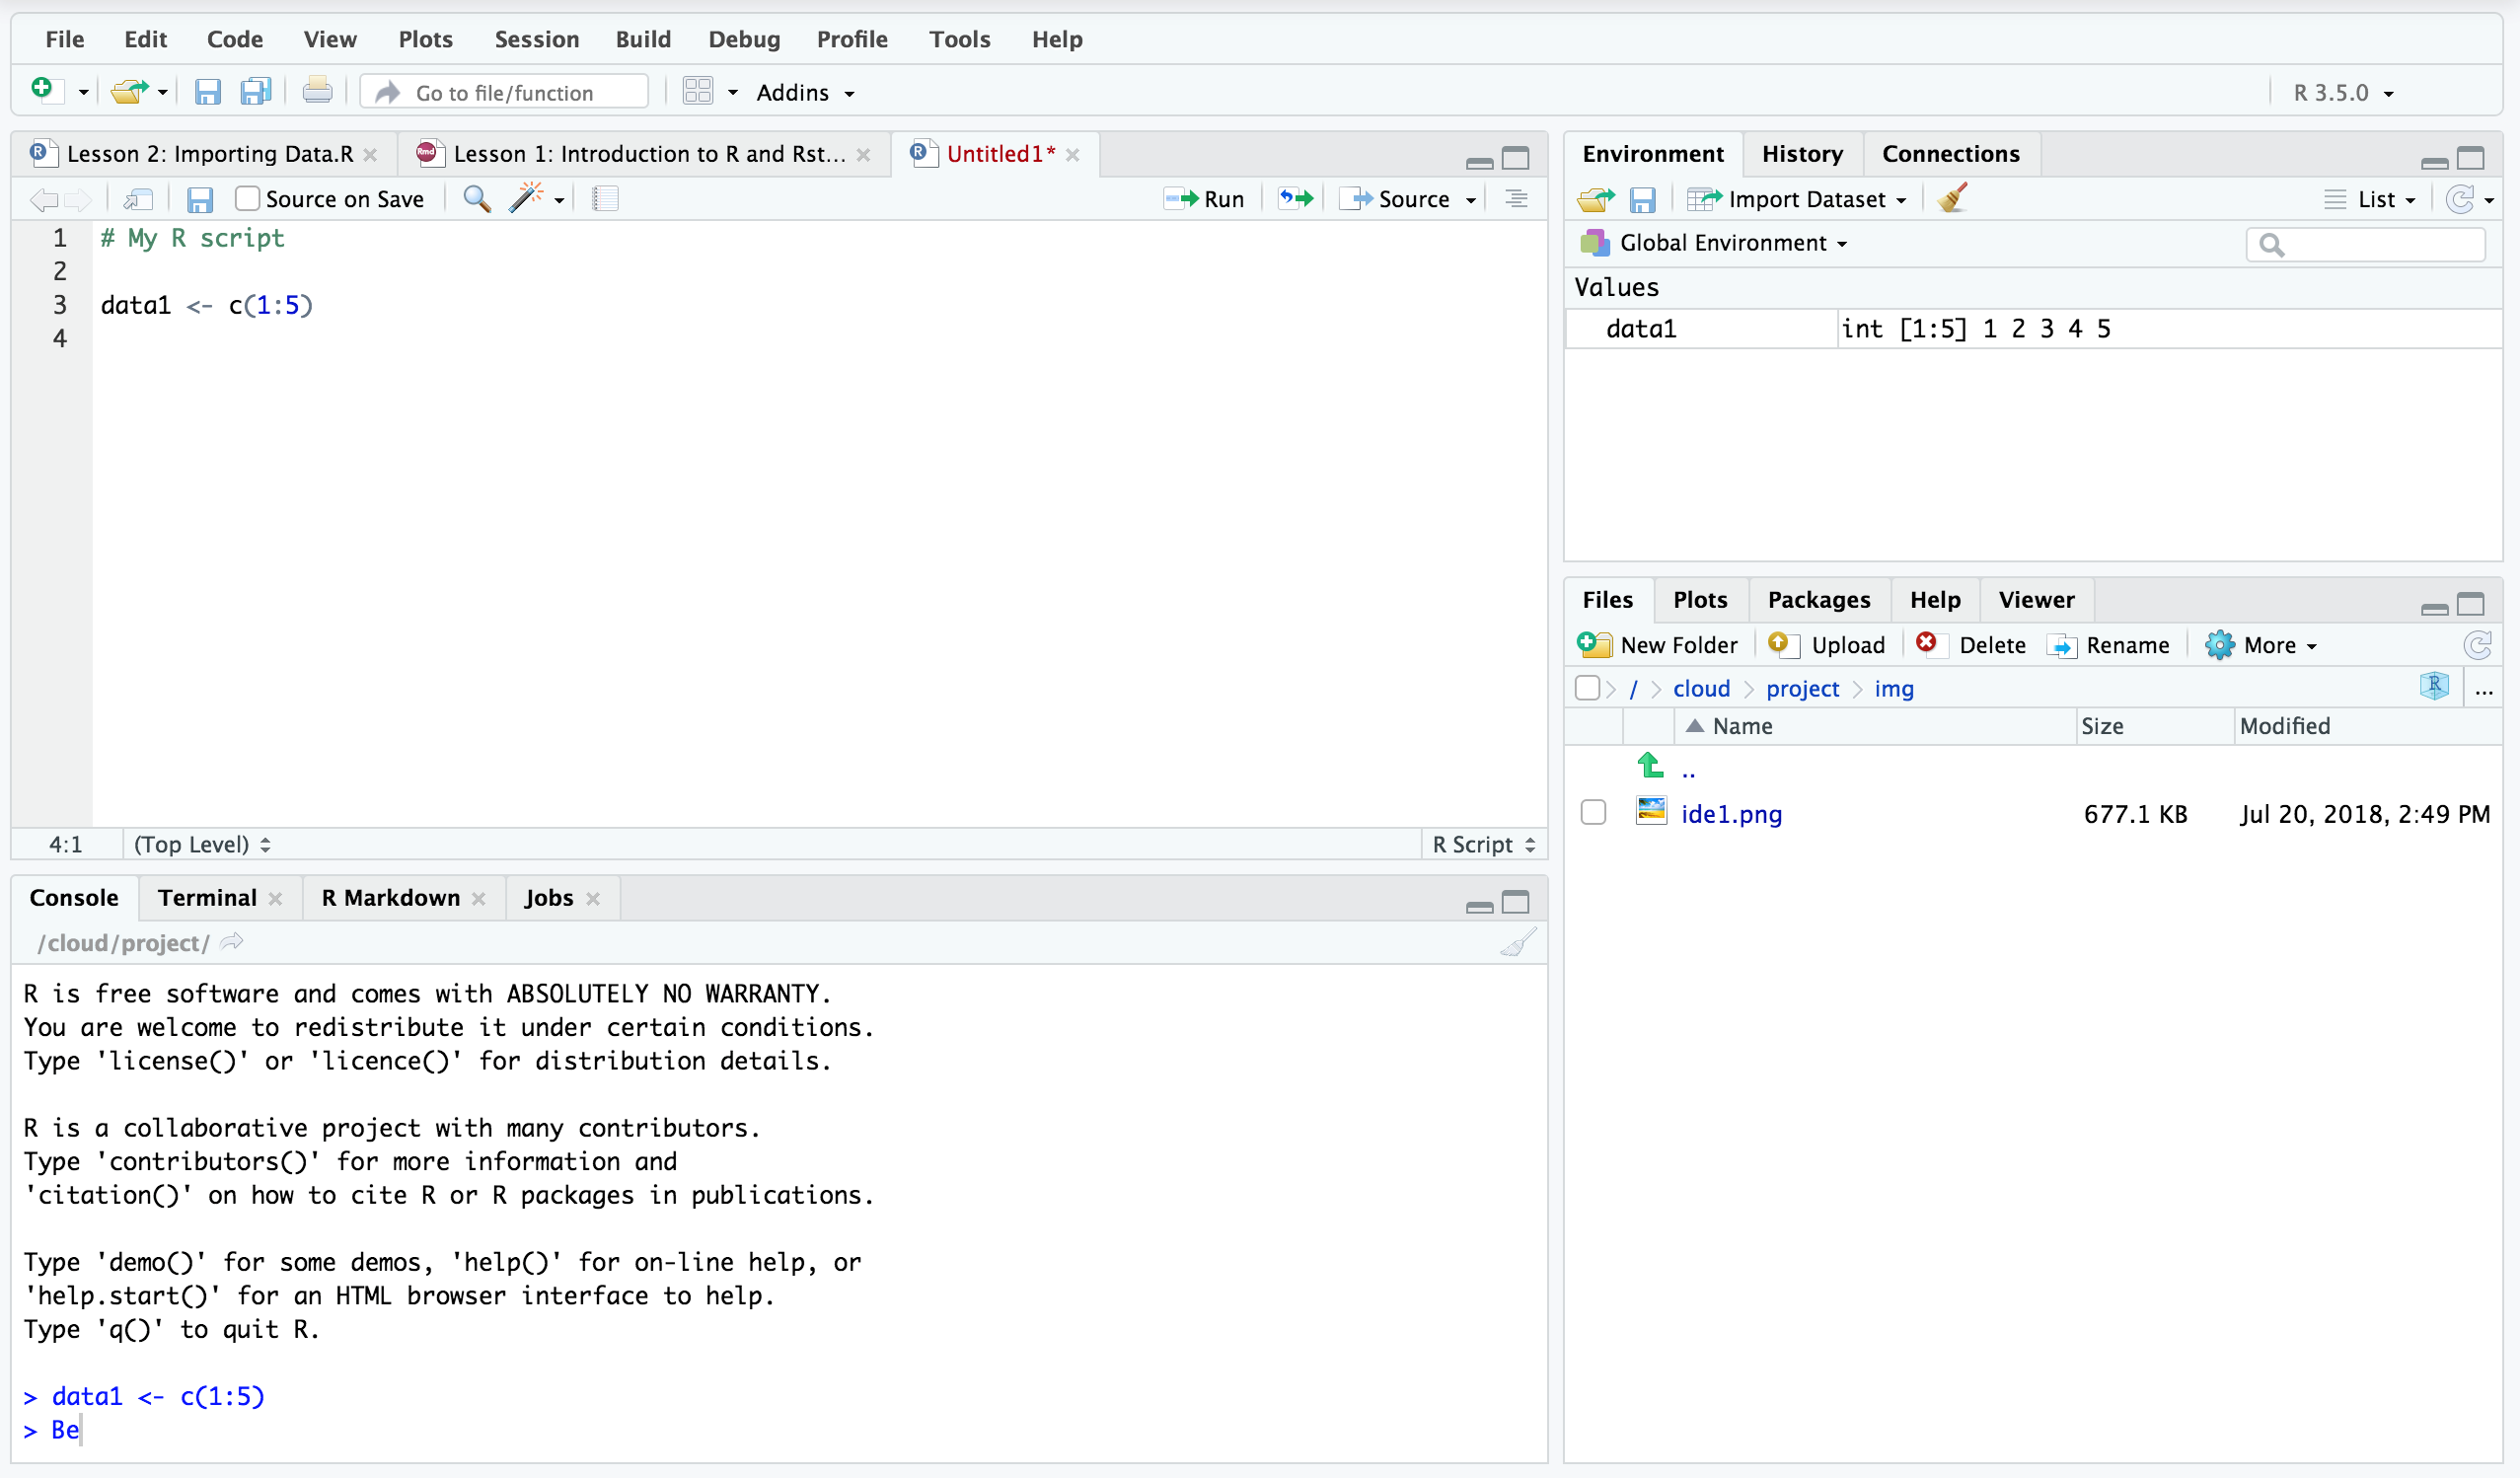
\includegraphics{images/rstudio1.png}

The interface for R Studio looks daunting at first. However, there are 4 main sections, 2 on the left and 2 on the right.

\begin{itemize}
\tightlist
\item
  MAIN TOP: R Script files or R Document Files

  \begin{itemize}
  \tightlist
  \item
    Where we usually type our code as a script before we run it. Script files are usually saved so we can work on them and rerun the code again later (.R files).
  \end{itemize}
\item
  MAIN BOTTOM: Console

  \begin{itemize}
  \tightlist
  \item
    Shows the output of our R code. We can type R code directly into the console and the answer will ouput immediately. However, it is more convenient to use script files.
  \end{itemize}
\item
  RIGHT TOP: Environment

  \begin{itemize}
  \tightlist
  \item
    Contains all of the objects (e.g.~data, analysis, equations, plots) that are currently stored in memory. We can save all of this to a file and load it later (.RData files).
  \end{itemize}
\item
  RIGHT BOTTOM: File Browser

  \begin{itemize}
  \tightlist
  \item
    The folder that R is working from is called `the working directory' and it will automatically look for files there if we try to import something (e.g.~a data file). Using the more button on the file browser allows you to set your desired working directory.
  \end{itemize}
\end{itemize}

\hypertarget{working-with-a-script}{%
\section{Working with a script}\label{working-with-a-script}}

Scripts can be opened from the \textbf{File} menu.

\begin{figure}
\centering
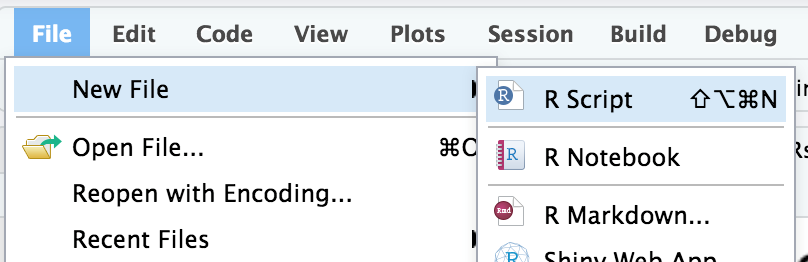
\includegraphics{images/file.png}
\caption{Creating a new script}
\end{figure}

The purpose of scripts is to allow you to type your analysis code and save it for use later. Scripts include, for example:

\begin{itemize}
\tightlist
\item
  Code for importing data into R
\item
  Your analysis code (e.g.~t-test or descriptive statistics)
\item
  Code for graphs and tables
\item
  Comments and notes (preceded by the `\#' symbol)
\end{itemize}

\begin{figure}
\centering
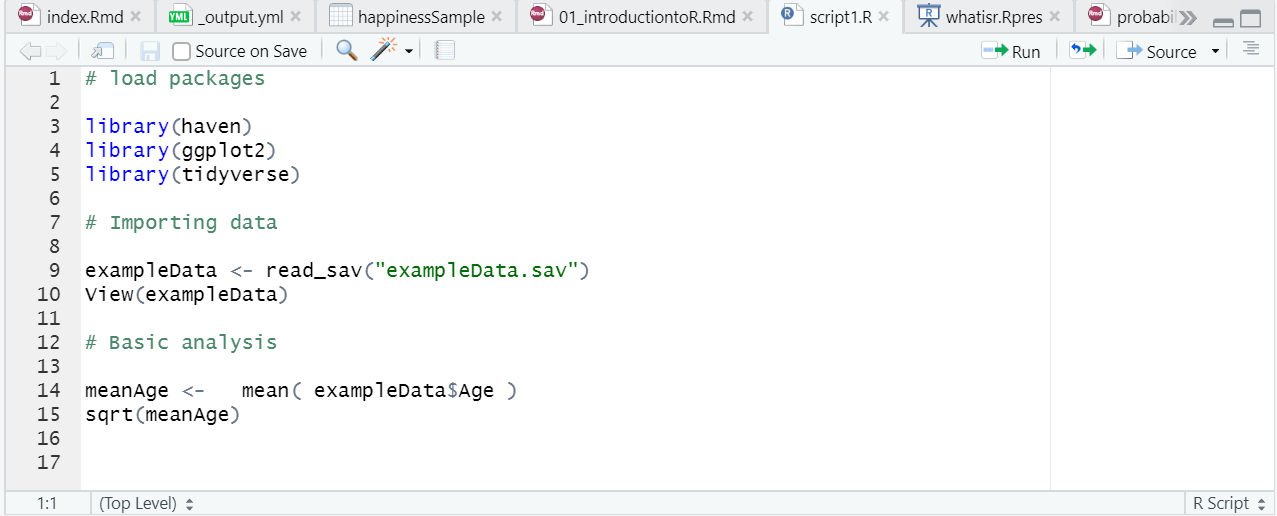
\includegraphics{images/script.png}
\caption{Example of an R script}
\end{figure}

To run a script, you click the \textbf{Run} button. You can choose to:

\begin{itemize}
\tightlist
\item
  Run the whole script
\item
  Run the selected line of code
\end{itemize}

\begin{figure}
\centering
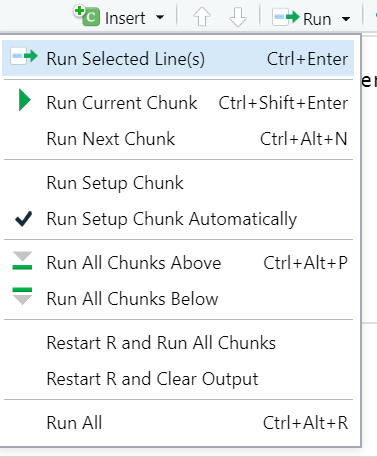
\includegraphics{images/run.png}
\caption{The run button}
\end{figure}

When you run the script, you will normally see output in the \textbf{console.}

\begin{figure}
\centering
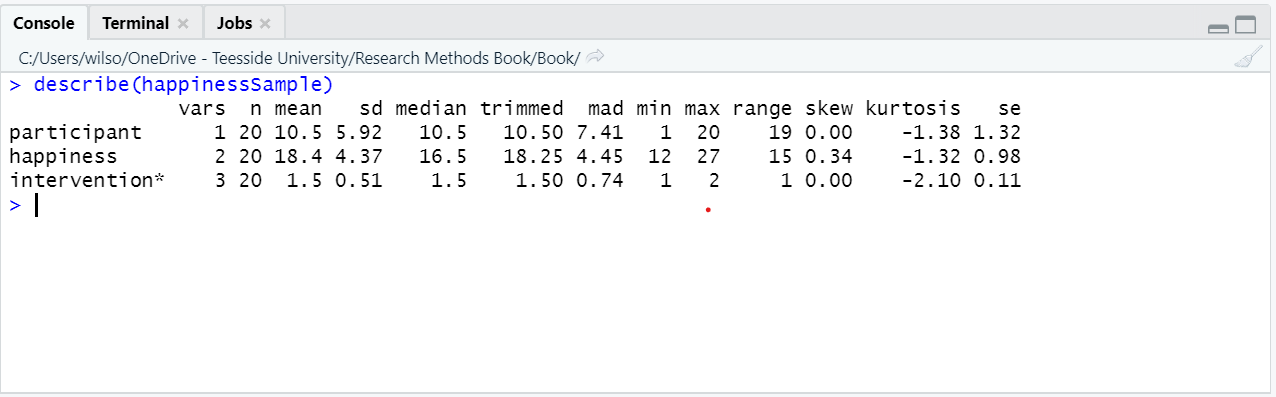
\includegraphics{images/console.png}
\caption{Output appears in the console}
\end{figure}

If your script contains code for a plot (graph), it will appear in the \textbf{Plots} window in the bottom right.

\begin{figure}
\centering
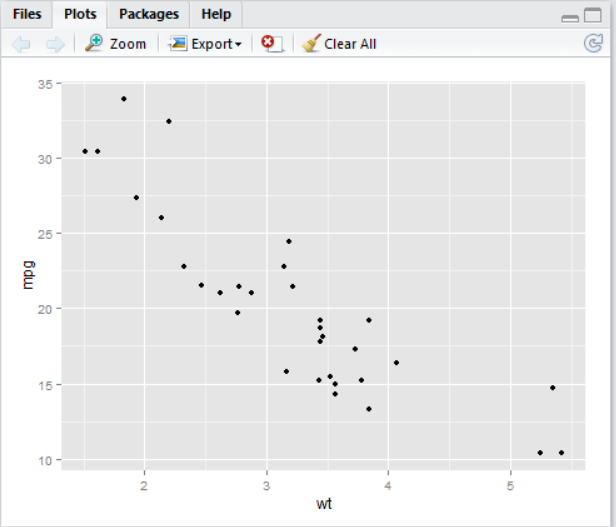
\includegraphics{images/plotwindow.png}
\caption{Plots appear in the plot window}
\end{figure}

\hypertarget{installing-and-loading-packages}{%
\section{Installing and loading packages}\label{installing-and-loading-packages}}

install Packages from RStudio, Inc. on Vimeo.

Packages add functionality to R and allow us to do new types of analysis.

\begin{itemize}
\item
  They can be installed via the menu (Tools -\textgreater{} Install Packages)
\item
  The can also be installed using code:

\begin{verbatim}
    install.packages()
\end{verbatim}
\end{itemize}

For example, TidyR is a package that contains functions for sorting and organising data. To install the package:

\begin{figure}
\centering
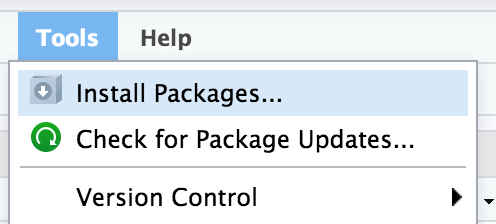
\includegraphics{images/installPackages.png}
\caption{Installing a package in RStudio}
\end{figure}

or use the code:

\begin{verbatim}
install.packages(“tidyr”)
\end{verbatim}

Once a package is has been installed, you need tp load it using the \emph{library()} command.
For example:

\begin{verbatim}
library(“tidyr”)
\end{verbatim}

\hypertarget{working-with-data-in-r}{%
\chapter{Working with data in R}\label{working-with-data-in-r}}

\hypertarget{by-the-end-of-this-section-you-will-be-able-to}{%
\section{By the end of this section, you will be able to:}\label{by-the-end-of-this-section-you-will-be-able-to}}

\begin{itemize}
\tightlist
\item
  Import data into R from excel, SPSS and csv files
\item
  Save data to objects
\item
  Identify different data structures and variable types
\item
  Convert variables from one type to another
\item
  Order, filter and group data
\item
  Summarise data
\item
  Create new variables from data
\end{itemize}

\hypertarget{in-this-section-we-will-use-the-tidyverse-set-of-packages}{%
\section{In this section, we will use the Tidyverse set of packages}\label{in-this-section-we-will-use-the-tidyverse-set-of-packages}}

\begin{itemize}
\tightlist
\item
  A `toolkit' of packages that are very useful for organsing and manipulating data
\item
  We will use the haven package to import SPSS files
\item
  We will use the dplyr to organise data
\item
  Also includes the ggplot2 and tidyR packages which we will use later
\end{itemize}

To install:

\begin{verbatim}
install.packages(“tidyverse”)
\end{verbatim}

(See the previous section on installing packages)

\hypertarget{import-data-into-r-from-excel-spss-and-csv-files}{%
\section{Import data into R from excel, SPSS and csv files}\label{import-data-into-r-from-excel-spss-and-csv-files}}

We can import data from a range of sources using the \textbf{Import Dataset} button in the \textbf{Environment} tab:

\begin{figure}
\centering
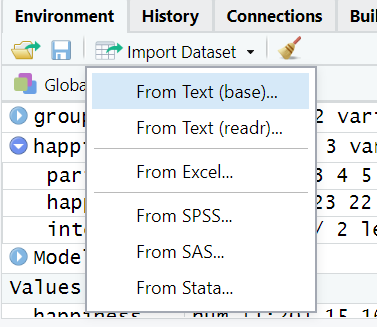
\includegraphics{images/importData.png}
\caption{Importing data}
\end{figure}

It is also possible to import data using code, for example:

\begin{verbatim}
# importing a .csv file
library(readr)
studentData <- read_csv("Datasets/studentData.csv")


#importing an SPSS file
library(haven)
mySPSSData <- read_sav("Datasets/salesData.sav")
\end{verbatim}

Once the data are imported, it will be visible in the environment:

\begin{figure}
\centering
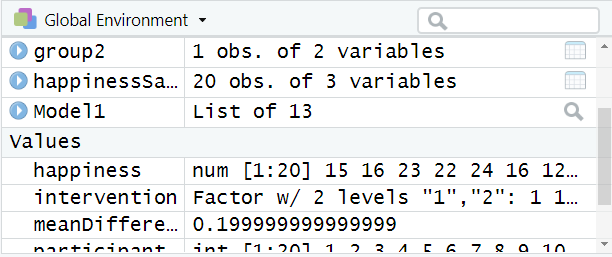
\includegraphics{images/environment.png}
\caption{Imported data in the environment}
\end{figure}

\hypertarget{understanding-objects-in-r}{%
\section{Understanding objects in R}\label{understanding-objects-in-r}}

In R, an \textbf{object} is anything that is saved to memory. For example, we might do some analysis:

\begin{verbatim}
mean(happiness)
\end{verbatim}

However, in the example above, the result would appear in the console but not be saved anywhere. To store the result for reuse later, we save it to an object:

\begin{verbatim}
happinessMean <- mean(happiness)
\end{verbatim}

In the above code (reading left to right):

\begin{itemize}
\tightlist
\item
  We name the object ``happinessMean''. This name can be anything we want.
\item
  The arrow means that the result of the code on the right will be saved to the object on the left.
\item
  The code on the right of the arrow calculates the mean of \emph{happiness} data
\end{itemize}

When this code is run, \emph{happinessMean} will be stored in the environment window:

\begin{figure}
\centering
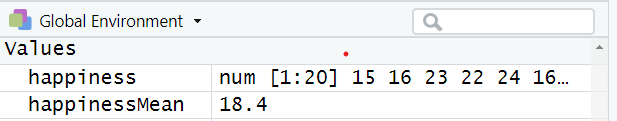
\includegraphics{images/saveobject.png}
\caption{Result of a calculation in the environment}
\end{figure}

To recall an object from the environment, we can simply type its name. For example:

\begin{verbatim}
happinessMean 
\end{verbatim}

\begin{quote}
Its important to note that anything can be stored as an object in R and recalled later. This includes, dataframes, the results of statistical calculations, plots etc.
\end{quote}

\hypertarget{identify-different-data-structures-and-variable-types}{%
\section{Identify different data structures and variable types}\label{identify-different-data-structures-and-variable-types}}

\hypertarget{data-structures}{%
\subsection{Data structures}\label{data-structures}}

There are many different types of data that R can work with. The most common type of data for most people tends to be a \textbf{dataframe}. A \textbf{dataframe} is what you might consider a ``normal'' 2-dimensional dataset, with rows of data and columns of variables:

\begin{figure}
\centering
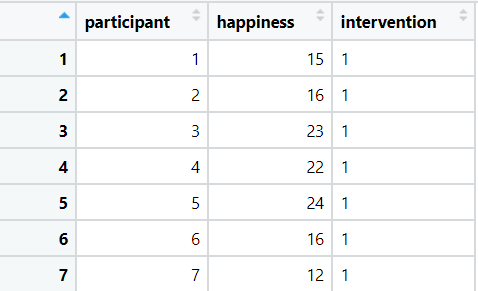
\includegraphics{images/dataframe.png}
\caption{A dataframe example}
\end{figure}

R can also use other data types.

A vector is a one-dimensional set of values:

\begin{Shaded}
\begin{Highlighting}[]
\CommentTok{# a vector example}

\NormalTok{scores <-}\StringTok{ }\KeywordTok{c}\NormalTok{(}\DecValTok{1}\NormalTok{,}\DecValTok{4}\NormalTok{,}\DecValTok{6}\NormalTok{,}\DecValTok{8}\NormalTok{,}\DecValTok{3}\NormalTok{,}\DecValTok{4}\NormalTok{,}\DecValTok{6}\NormalTok{,}\DecValTok{7}\NormalTok{)}
\end{Highlighting}
\end{Shaded}

A matrix is a multi-dimensional set of values. The below example is a 3-dimensional matrix, there are 2 groups of 2 rows and 3 columns:

\begin{verbatim}
## , , 1
## 
##      [,1] [,2] [,3]
## [1,]    1    3    5
## [2,]    2    4    6
## 
## , , 2
## 
##      [,1] [,2] [,3]
## [1,]    7    9   11
## [2,]    8   10   12
\end{verbatim}

\begin{quote}
We will primarily work with dataframes (and sometimes vectors), as this is how the data in psychology research is usually structured.
\end{quote}

\hypertarget{variable-types}{%
\subsection{Variable types}\label{variable-types}}

With numerical data, there are 4 key data types:

\begin{itemize}
\tightlist
\item
  Nominal (a category, group or factor)
\item
  Ordinal (a ranking)
\item
  Interval (scale data that can include negative values)
\item
  Ratio (scale data that cannot include negative values)
\end{itemize}

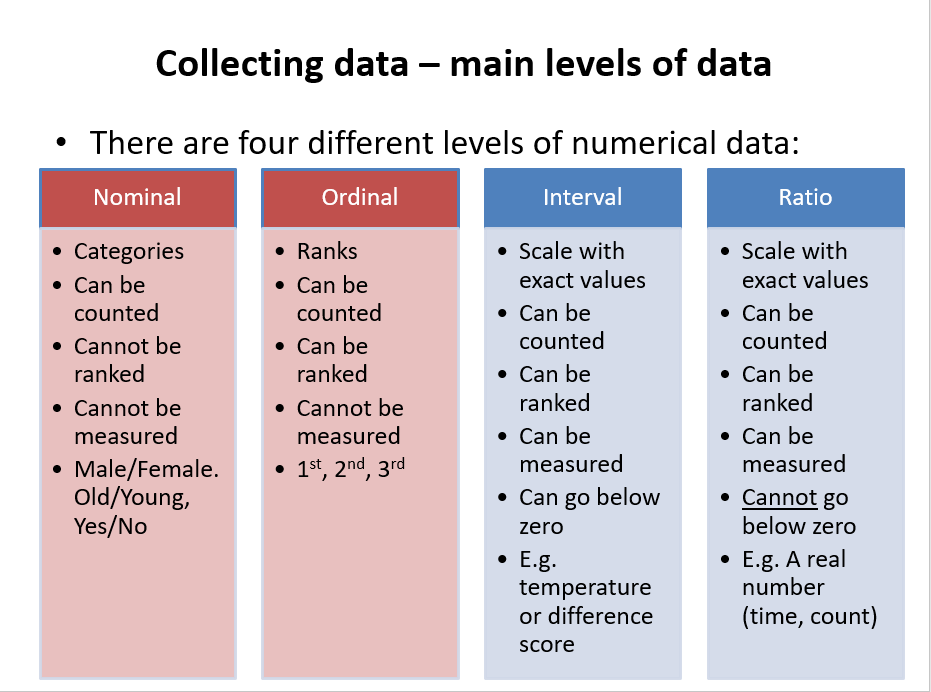
\includegraphics{images/dataTypes.png}
R can use all of these variable types:

\begin{itemize}
\tightlist
\item
  \textbf{Nominal} variables are called \textbf{factors}
\item
  \textbf{Ordinal} variables are called \textbf{ordered factors}
\item
  \textbf{Interval and ratio} variables are called \textbf{numeric} data and can sometimes be called integers (if they are only whole numbers) or doubles (if they all have decimal points)
\end{itemize}

R can also use other data types such as text (\textbf{character}) data.

\hypertarget{convert-variables-from-one-type-to-another}{%
\subsection{Convert variables from one type to another}\label{convert-variables-from-one-type-to-another}}

When we first import data into R, it might not recognise the data types correctly. For example, in the below data, we can see the \textbf{intervention} variable :

\begin{verbatim}
##    participant intervention happiness
## 1            1            1  6.785931
## 2           20            1  6.878551
## 3           13            2  7.494531
## 4           14            2  7.549832
## 5           12            2  8.295756
## 6           10            1  8.986315
## 7            2            1  9.139099
## 8           16            2  9.236834
## 9            5            2  9.527681
## 10           9            2  9.592461
\end{verbatim}

In the \textbf{intervention} variable, the numbers 1 and 2 refer to different intervention groups. Therefore, the variable is a \textbf{factor} variable. To ensure that R understands this, we can resave the intervention variable as a factor using the \emph{as.factor()} function:

\begin{Shaded}
\begin{Highlighting}[]
\NormalTok{happinessSample}\OperatorTok{$}\NormalTok{intervention <-}\StringTok{ }\KeywordTok{as.factor}\NormalTok{(happinessSample}\OperatorTok{$}\NormalTok{intervention)}
\end{Highlighting}
\end{Shaded}

\hypertarget{working-with-dataframes}{%
\section{Working with dataframes}\label{working-with-dataframes}}

Dataframes are the more standard data format that were are used to (think of how a dataset looks in SPSS or Excel).

In a dataframe, variables are columns and each row usually reperesents one measurement or one participant.

\hypertarget{view-dataframe}{%
\subsection{View dataframe}\label{view-dataframe}}

To view a dataframe, we can click on it in the environment window and it will display:

\begin{figure}
\centering
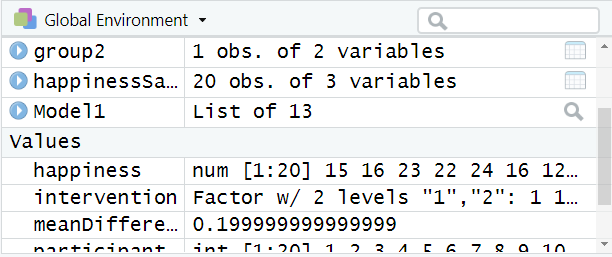
\includegraphics{images/environment.png}
\caption{Clicking on datasets in hte environment will open them up for viewing}
\end{figure}

\begin{figure}
\centering
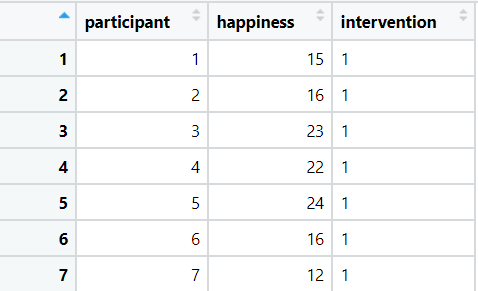
\includegraphics{images/dataframe.png}
\caption{Viewing a dataframe}
\end{figure}

\hypertarget{refer-to-variables-columns-in-a-dataframe}{%
\subsection{Refer to variables (columns) in a dataframe}\label{refer-to-variables-columns-in-a-dataframe}}

Columns in a dataframe are accessed using the ``\$'' sign. For example, to access the \emph{happiness} column in the \emph{happinessSample} dataframe, we would type:

\begin{Shaded}
\begin{Highlighting}[]
\NormalTok{happinessSample}\OperatorTok{$}\NormalTok{happiness}
\end{Highlighting}
\end{Shaded}

\begin{verbatim}
##  [1]  6.785931  9.139099 11.319182 11.873362  9.527681  9.950592  9.841057 10.584258  9.592461
## [10]  8.986315 12.965060  8.295756  7.494531  7.549832 11.049785  9.236834 11.613146  9.635646
## [19] 12.127610  6.878551
\end{verbatim}

As we can see above, the result is then displayed.

\hypertarget{order-filter-and-group-data}{%
\subsection{Order, filter and group data}\label{order-filter-and-group-data}}

If you have the \textbf{tidyverse} package loaded, it is easy to organise and filter data.

\begin{Shaded}
\begin{Highlighting}[]
\KeywordTok{arrange}\NormalTok{(happinessSample, happiness)}
\end{Highlighting}
\end{Shaded}

\begin{verbatim}
##    participant intervention happiness
## 1            1            1  6.785931
## 2           20            1  6.878551
## 3           13            2  7.494531
## 4           14            2  7.549832
## 5           12            2  8.295756
## 6           10            1  8.986315
## 7            2            1  9.139099
## 8           16            2  9.236834
## 9            5            2  9.527681
## 10           9            2  9.592461
## 11          18            2  9.635646
## 12           7            2  9.841057
## 13           6            1  9.950592
## 14           8            1 10.584258
## 15          15            1 11.049785
## 16           3            2 11.319182
## 17          17            2 11.613146
## 18           4            1 11.873362
## 19          19            2 12.127610
## 20          11            2 12.965060
\end{verbatim}

\begin{Shaded}
\begin{Highlighting}[]
\KeywordTok{arrange}\NormalTok{(happinessSample, }\KeywordTok{desc}\NormalTok{(happiness)) }\CommentTok{# Arrange in descending order}
\end{Highlighting}
\end{Shaded}

\begin{verbatim}
##    participant intervention happiness
## 1           11            2 12.965060
## 2           19            2 12.127610
## 3            4            1 11.873362
## 4           17            2 11.613146
## 5            3            2 11.319182
## 6           15            1 11.049785
## 7            8            1 10.584258
## 8            6            1  9.950592
## 9            7            2  9.841057
## 10          18            2  9.635646
## 11           9            2  9.592461
## 12           5            2  9.527681
## 13          16            2  9.236834
## 14           2            1  9.139099
## 15          10            1  8.986315
## 16          12            2  8.295756
## 17          14            2  7.549832
## 18          13            2  7.494531
## 19          20            1  6.878551
## 20           1            1  6.785931
\end{verbatim}

\begin{itemize}
\tightlist
\item
  Show clients with a happiness score of less than 4
\end{itemize}

\begin{Shaded}
\begin{Highlighting}[]
\KeywordTok{filter}\NormalTok{(happinessSample, happiness }\OperatorTok{<}\StringTok{ }\DecValTok{4}\NormalTok{)}
\end{Highlighting}
\end{Shaded}

\begin{verbatim}
## [1] participant  intervention happiness   
## <0 rows> (or 0-length row.names)
\end{verbatim}

\begin{itemize}
\tightlist
\item
  Show Intervention group 2 with happiness scores above 7
\end{itemize}

\begin{Shaded}
\begin{Highlighting}[]
\KeywordTok{filter}\NormalTok{(happinessSample, happiness }\OperatorTok{>}\StringTok{ }\DecValTok{7} \OperatorTok{&}\StringTok{ }\NormalTok{intervention }\OperatorTok{==}\StringTok{ }\DecValTok{2}\NormalTok{)}
\end{Highlighting}
\end{Shaded}

\begin{verbatim}
##    participant intervention happiness
## 1            3            2 11.319182
## 2            5            2  9.527681
## 3            7            2  9.841057
## 4            9            2  9.592461
## 5           11            2 12.965060
## 6           12            2  8.295756
## 7           13            2  7.494531
## 8           14            2  7.549832
## 9           16            2  9.236834
## 10          17            2 11.613146
## 11          18            2  9.635646
## 12          19            2 12.127610
\end{verbatim}

\begin{itemize}
\tightlist
\item
  Group by intervention and show the mean happiness score
\end{itemize}

\begin{Shaded}
\begin{Highlighting}[]
\NormalTok{happinessSample }\OperatorTok\StringTok{ }\KeywordTok{group_by}\NormalTok{(intervention) }\OperatorTok\StringTok{ }\KeywordTok{summarise}\NormalTok{(}\DataTypeTok{mean =} \KeywordTok{mean}\NormalTok{(happiness))}
\end{Highlighting}
\end{Shaded}

\begin{verbatim}
## `summarise()` ungrouping output (override with `.groups` argument)
\end{verbatim}

\begin{verbatim}
## # A tibble: 2 x 2
##   intervention  mean
##   <fct>        <dbl>
## 1 1             9.41
## 2 2             9.93
\end{verbatim}

\hypertarget{create-new-variables-from-data}{%
\subsection{Create new variables from data}\label{create-new-variables-from-data}}

To create new variables from data, we can use the \textbf{mutate()} function.

For example, let's say we wanted to calculate the difference between each person's happiness score and the mean happiness score.

We could do the following:

\begin{Shaded}
\begin{Highlighting}[]
\NormalTok{happinessSample }\OperatorTok\StringTok{ }\KeywordTok{mutate}\NormalTok{(}\DataTypeTok{difference =}\NormalTok{ happiness }\OperatorTok{-}\StringTok{ }\KeywordTok{mean}\NormalTok{(happiness))}
\end{Highlighting}
\end{Shaded}

\begin{verbatim}
##    participant intervention happiness  difference
## 1            1            1  6.785931 -2.93640295
## 2            2            1  9.139099 -0.58323556
## 3            3            2 11.319182  1.59684776
## 4            4            1 11.873362  2.15102748
## 5            5            2  9.527681 -0.19465333
## 6            6            1  9.950592  0.22825761
## 7            7            2  9.841057  0.11872229
## 8            8            1 10.584258  0.86192386
## 9            9            2  9.592461 -0.12987337
## 10          10            1  8.986315 -0.73601959
## 11          11            2 12.965060  3.24272524
## 12          12            2  8.295756 -1.42657888
## 13          13            2  7.494531 -2.22780305
## 14          14            2  7.549832 -2.17250279
## 15          15            1 11.049785  1.32745030
## 16          16            2  9.236834 -0.48550020
## 17          17            2 11.613146  1.89081116
## 18          18            2  9.635646 -0.08668862
## 19          19            2 12.127610  2.40527587
## 20          20            1  6.878551 -2.84378324
\end{verbatim}

  \bibliography{book.bib,packages.bib}

\end{document}
